\section{Comparaison des bibliothèques d'intelligence artificielle}
\label{sec:comparaisonIA}

\subsection{Objectifs}
\label{sec:comparaisonIA:objectifs}

L'objectif de cette étude est de comparer plusieurs bibliothèques d'intelligence artificielle
permettant de détecter des cyclistes à partir d'une vidéo.

\subsection{Méthode de recherche}
\label{sec:comparaisonIA:methode_recherche}

Après quelques recherches, nous avons trouvé 2 bibliothèques d'intelligence artificielle
qui permettent de détecter des objets à partir d'une vidéo : ImageAI et OpenCV.
Elles fonctionnent avec le langage de programmation Python.

\subsubsection{ImageAI}
\label{sec:comparaisonIA:methode_recherche:imageAI}

ImageAI dispose de fonctions déjà prêtes pour réaliser de la détection d'objets dans une vidéo.
Avec cette bibliothèque, cette détection est possible avec un code d'une dizaine de lignes.
Elle offre le choix de la vitesse de détection : normal, fast, faster, fastest et flash.

\subsubsection{OpenCV}
\label{sec:comparaisonIA:methode_recherche:openCV}

OpenCV laisse au codeur le soin de récupérer la position des objets, leur probabilité, et de dessiner un cadre autour de ces objets.
Avec cette bibliothèque, une cinquantaine de lignes de code est nécessaire.
Elle propose d'utiliser un algorithme étant entraîné à différentes tailles d'images : (320px, 320px), (416px, 416px) ou (608px, 608px).

\subsubsection{Règles à suivre par les programmes}
\label{sec:comparaisonIA:methode_recherche:regles}
Dans un premier temps, nous avons testé des programmes utilisant les bibliothèques ImageAI et OpenCV \cite{ImageAI, OpenCV}.
Puis, nous avons adapté ces programmes à nos besoins.
Afin de pouvoir comparer ces 2 bibliothèques, nous avons fixé les règles que nos 2 programmes doivent suivre :

\begin{itemize}
    \item Détecter seulement les cyclistes et ignorer les autres objets
    \item Considérer que les cyclistes sont détectés lorsqu'ils le sont avec une probabilité de minimum 50\%
    \item Lorsqu'un cycliste est détecté, afficher un message dans la console avec la probabilité associée
    \item Réaliser un fichier vidéo de sortie au format "avi" ayant une image par seconde, et contenant des cadres autour des cyclistes détectés avec leur probabilité associée
    \item Utiliser l'algorithme d'intelligence artificielle YOLOv3
\end{itemize}

\subsubsection{L'algorithme YOLO}
\label{sec:comparaisonIA:methode_recherche:yolo}

YOLO est l'acronyme de "You Only Look Once". Cela traduit le fait qu'un seul réseau de neurone est utilisé. \cite{Yolov3}
Ce dernier divise les images d'une vidéo en régions, et prédit des cadres contenant des objets avec leur probabilité pour chaque région.
Ensuite, seuls les cadres contenant des objets avec une probabilité assez forte sont conservés.
Nous utilisons la version 3 de YOLO qui date de 2018, car celle-ci est à la fois supportée par ImageAI et OpenCV.

\subsubsection{Méthode de comparaison}
\label{sec:comparaisonIA:methode_recherche:methode_comparaison}

Nous avons comparé nos 2 programmes utilisant respectivement les bibliothèques ImageAI et OpenCV avec leurs différents paramètres.
Le programme utilisant ImageAI a donc été testé avec ses différentes vitesses de détection : normal, fast, fastest et flash.
La vitesse "faster" a été écartée car elle ne permettait pas de détecter de vélo sur notre vidéo de référence.
De même, le programme utilisant OpenCV a été testé avec un algorithme étant entraîné à différentes tailles d'images :
(320px, 320px), (416px, 416px) et (608px, 608px).

La \gls{video de reference} que nous avons utilisée est une vidéo de 15 secondes suivant un cycliste sur une route.
Lorsque nous effections des tests avec la vidéo originale ayant 30 images par seconde (ips),
le temps de traitement de cette vidéo dépassait les 3 minutes.
Nous avons donc choisi de tester cette vidéo avec 1 ips, 2 ips et 3 ips.

Pour comparer nos 2 programmes avec leurs différents paramètres, nous avons réalisé un programme en Python permettant
d'exécuter ces programmes tout en calculant leur temps d'exécution.
Cela affiche ensuite ces différents temps sous la forme d'un diagramme en bâtons grâce à la bibliothèque matplotlib.
Nous avons également réalisé un tableau montrant l'efficacité des 2 programmes suivant leurs différents paramètres.

Ces tests ont été réalisé à partir d'un ordinateur ayant les paramètres suivant :
\begin{itemize}
    \item Type : VivoBook\_ASUSLaptop X521FA\_K533FA 1.0
    \item Système d'exploitation utilisé : Linux
    \item Distribution utilisée : Ubuntu 20.04.3 LTS x86\_64
    \item \gls{CPU} : Intel i7-10510U (8) @ 4.900GHz
    \item \gls{GPU} : Intel CometLake-U GT2 [UHD Graphics]
\end{itemize}
Il est à noter que cet ordinateur ne dispose pas de GPU NVIDIA, ce qui aurait augmenté la rapidité des tests.

\subsection{Résultats}
\label{sec:comparaisonIA:resultats}

\subsubsection{Comparaison à 1'image par seconde}
\label{sec:comparaisonIA:resultats:1fps}

\begin{figure}[H]
    \centering
    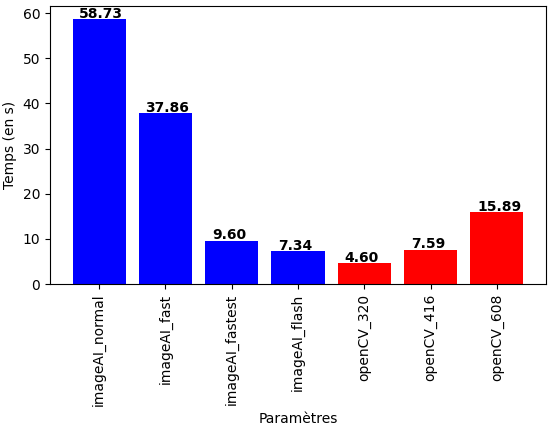
\includegraphics[width=0.7\textwidth]{img/result_1fps.png}
    \caption{Comparaison des bibliothèques ImageAI et OpenCV à 1 ips}
\end{figure}

Le tableau~\ref{tab_1fps} présente l'efficacité des 2 programmes suivant leurs différents paramètres à 1 ips.
Il renseigne le nombre de fois que le vélo a été détecté sur la vidéo ayant 1 ips.
Lorsque le vélo est détecté 2 fois sur une image, cela n'est pas pris en compte dans le nombre de détections.
Cependant, cela apparaît dans la colonne "Détection en double".

\begin{table}[H]
    \centering
    \rowcolors{2}{tableColor}{white}
    \begin{tabular}{|c|c|c|c|}
        \hline
        \rowcolor{tableColorDark} Paramètres & Nb de détections & Détection en double \\
        \hline

        imageAI\_normal                      & 9                & 1                   \\\hline
        imageAI\_fast                        & 8                & 0                   \\\hline
        imageAI\_fastest                     & 6                & 0                   \\\hline
        imageAI\_flash                       & 5                & 0                   \\\hline
        openCV\_320                          & 9                & 0                   \\\hline
        openCV\_416                          & 9                & 0                   \\\hline
        openCV\_608                          & 8                & 1                   \\\hline
    \end{tabular}
    \caption{Comparaison de l'efficacité des 2 programmes suivant leurs différents paramètres à 1 ips}
    \label{tab_1fps}
\end{table}

\subsubsection{Comparaison à 2 images par seconde}
\label{sec:comparaisonIA:resultats:2fps}

\begin{figure}[H]
    \centering
    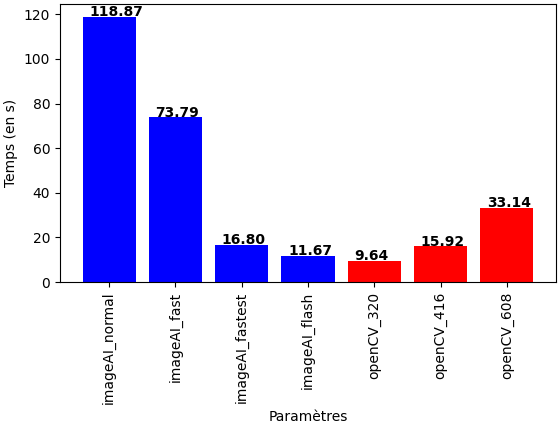
\includegraphics[width=0.7\textwidth]{img/result_2fps.png}
    \caption{Comparaison des bibliothèques ImageAI et OpenCV à 2 ips}
\end{figure}

Le tableau~\ref{tab_2fps} présente l'efficacité des 2 programmes suivant leurs différents paramètres à 2 ips.
Il renseigne le nombre de fois que le vélo a été détecté sur la vidéo ayant 2 ips.
Lorsque le vélo est détecté 2 fois sur une image, cela n'est pas pris en compte dans le nombre de détections.
Cependant, cela apparaît dans la colonne "Détection en double".

\begin{table}
    \begin{center}
        \rowcolors{2}{tableColor}{white}
        \begin{tabular}{|c|c|c|c|}
            \hline
            \rowcolor{tableColorDark} Paramètres & Nb de détections & Détection en double \\
            \hline

            imageAI\_normal                      & 14               & 1                   \\\hline
            imageAI\_fast                        & 14               & 0                   \\\hline
            imageAI\_fastest                     & 11               & 0                   \\\hline
            imageAI\_flash                       & 9                & 0                   \\\hline
            openCV\_320                          & 15               & 0                   \\\hline
            openCV\_416                          & 16               & 0                   \\\hline
            openCV\_608                          & 14               & 0                   \\\hline
        \end{tabular}
        \caption{Comparaison de l'efficacité des 2 programmes suivant leurs différents paramètres à 2 ips}
        \label{tab_2fps}
    \end{center}
\end{table}

\subsubsection{Comparaison à 3 images par seconde}
\label{sec:comparaisonIA:resultats:3fps}

\begin{figure}[H]
    \centering
    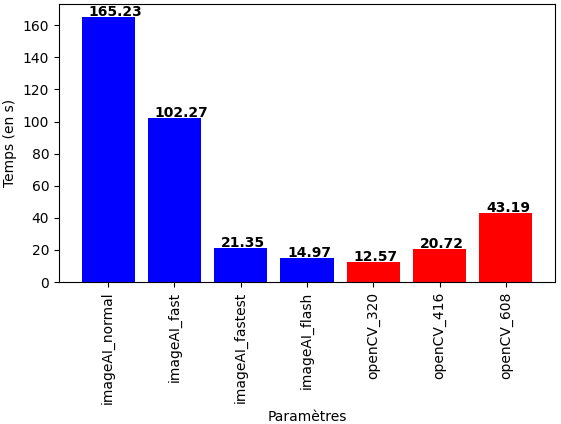
\includegraphics[width=0.7\textwidth]{img/result_3fps.png}
    \caption{Comparaison des bibliothèques ImageAI et OpenCV à 3 ips}
\end{figure}

Le tableau~\ref{tab_3fps} présente l'efficacité des 2 programmes suivant leurs différents paramètres à 3 ips.
Il renseigne le nombre de fois que le vélo a été détecté sur la vidéo ayant 3 ips.
Lorsque le vélo est détecté 2 fois sur une image, cela n'est pas pris en compte dans le nombre de détections.
Cependant, cela apparaît dans la colonne "Détection en double".

\begin{table}
    \centering
    \rowcolors{2}{tableColor}{white}
    \begin{tabular}{|c|c|c|c|}
        \hline
        \rowcolor{tableColorDark} Paramètres & Nb de détections & Détection en double \\
        \hline

        imageAI\_normal                      & 20               & 1                   \\\hline
        imageAI\_fast                        & 20               & 0                   \\\hline
        imageAI\_fastest                     & 16               & 0                   \\\hline
        imageAI\_flash                       & 13               & 0                   \\\hline
        openCV\_320                          & 21               & 0                   \\\hline
        openCV\_416                          & 22               & 0                   \\\hline
        openCV\_608                          & 22               & 0                   \\\hline
    \end{tabular}
    \caption{Comparaison de l'efficacité des 2 programmes suivant leurs différents paramètres à 3 ips}
    \label{tab_3fps}
\end{table}

\subsection{Conclusion}
\label{sec:comparaisonIA:conclusion}

Les 3 tests réalisés nous montrent que c'est la bibliothèque OpenCV,
associée à l'algorithme YOLOv3 étant entraîné aux images de taille (320px, 320px) qui est la plus rapide.
Ces paramètres font également partie de ceux présentant la meilleure efficacité en termes de nombre de détections du vélo.
Nous choisissons donc ces paramètres pour notre projet.
D'autres bibliothèques auraient pu être testées telles que GluonCV, PyTorch\dots
Cependant, OpenCV semble être suffisant pour répondre à nos besoins.
